\documentclass[12pt, twoside]{article}
\input{/Users/chris/github/course-files/docs/ib/preamble}

\fancyhead[LO]{La Scuola d'Italia / Dr.\ Huson / IB Math 12 HL \\* 15 September 2026}
\fancyhead[RO]{\fbox{\begin{minipage}{6cm}\footnotesize Nickname:\\[0.5cm]\end{minipage}}}
\fancyhead[LE]{\fbox{\begin{minipage}{6cm}\footnotesize Nickname:\\[0.5cm]\end{minipage}}}
\fancyfoot[C]{\thepage}

\begin{document}
\subsubsection*{12.4 Classwork: de Moivre, Trigonometric Identities and Roots of Unity (no calculator)}

Answer all three problems in the spaces provided. Show your working. Give all
answers as exact values (surds and fractions of $\pi$), not decimals.

\begin{enumerate}[itemsep=0.15cm]

%--- Problem 1: de Moivre + binomial expansion -> cos 3t = 4cos^3 t - 3cos t [6 marks] ---
%--- Source: authored 2026-09-15 (HL syllabus 1.14) ---
\item[1.]

Let $\theta$ be any real number.

\begin{enumerate}[itemsep=0.15cm]
  \item Use de Moivre's theorem to write $(\cos\theta + i\sin\theta)^{3}$ in
  terms of $\cos 3\theta$ and $\sin 3\theta$.
  \item Expand $(\cos\theta + i\sin\theta)^{3}$ using the binomial theorem,
  simplifying the powers of $i$.
  \item By equating real parts, show that
  $$\cos 3\theta = 4\cos^{3}\theta - 3\cos\theta.$$
\end{enumerate}

\begin{tikzpicture}
  \draw (-0.6,0) rectangle (14.6,13.6);
  \foreach \y in {1,2,...,12} \draw[dotted] (0,\y)--(14.1,\y);
\end{tikzpicture}

\newpage

%--- Problem 2: imaginary parts -> sin 3t, then solve 8c^3 - 6c = 1 [5 marks] ---
%--- Source: authored 2026-09-15 (HL syllabus 1.14, 1.9) ---
\item[2.]

\begin{enumerate}[itemsep=0.15cm]
  \item Using your expansion from Problem 1, equate imaginary parts to find an
  expression for $\sin 3\theta$ in terms of $\sin\theta$ only.
  \item Hence solve the equation
  $$8\cos^{3}\theta - 6\cos\theta = 1, \qquad 0 \leq \theta < \pi,$$
  giving all solutions as exact multiples of $\pi$.
\end{enumerate}

\begin{tikzpicture}
  \draw (-0.6,0) rectangle (14.6,15.2);
  \foreach \y in {1,2,...,14} \draw[dotted] (0,\y)--(14.1,\y);
\end{tikzpicture}

\newpage

%--- Problem 3: fifth roots of unity, sum zero, regular pentagon [5 marks] ---
%--- Source: authored 2026-09-15 (HL syllabus 1.14) ---
\item[3.]

Let $\omega$ be a complex number satisfying $\omega^{5} = 1$.

\begin{enumerate}[itemsep=0.15cm]
  \item Find all five solutions of $z^{5} = 1$, giving each in the form
  $e^{i\theta}$ with $-\pi < \theta \leq \pi$.
  \item Show that the five solutions sum to zero.
  \item The five solutions are plotted on an Argand diagram. Describe the
  figure they form, stating its centre and the distance of each vertex from
  the origin.
\end{enumerate}

\begin{center}
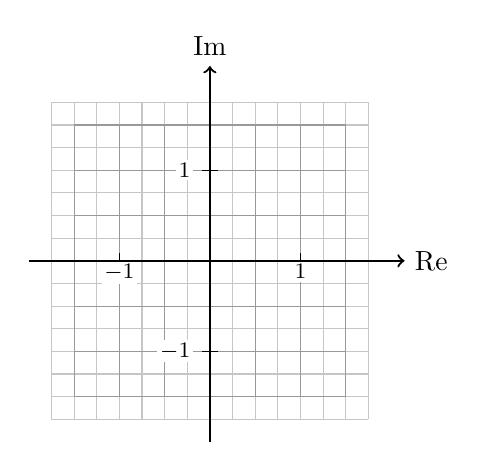
\begin{tikzpicture}[scale=1.15]
  \draw [thin, color=gray!45, step=0.25cm] (-1.75,-1.75) grid (1.75,1.75);
  \draw [thin, color=gray!80] (-1.5,-1.5) grid[step=0.5cm] (1.5,1.5);
  \draw [thick, ->] (-2.0,0) -- (2.15,0) node [right] {$\mathrm{Re}$};
  \draw [thick, ->] (0,-2.0) -- (0,2.15) node [above] {$\mathrm{Im}$};
  \foreach \x in {-1,1} \draw[shift={(\x,0)}] (0pt,-2.5pt) -- (0pt,2.5pt)
     node[below=3pt, fill=white, inner sep=1pt] {\footnotesize $\x$};
  \foreach \y in {-1,1} \draw[shift={(0,\y)}] (2.5pt,0pt) -- (-2.5pt,0pt)
     node[left=3pt, fill=white, inner sep=1pt] {\footnotesize $\y$};
\end{tikzpicture}
\end{center}

\begin{tikzpicture}
  \draw (-0.6,0) rectangle (14.6,10.4);
  \foreach \y in {1,2,...,9} \draw[dotted] (0,\y)--(14.1,\y);
\end{tikzpicture}

\end{enumerate}
\end{document}
